% ============================================================
% paper_ko.tex — paper.tex의 한국어 버전 (검토용, 제출용 아님)
% BMVC 제출은 paper.tex (영어)로 진행
% 컴파일러: XeLaTeX 또는 LuaLaTeX 필수 (kotex 때문)
% ============================================================

\documentclass{bmvc2k}

\bmvcreviewcopy{??}

\title{딥 ResNet이 학습에 성공하는 이유:\\
스킵 연결이 가능케 하는 효과적 깊이의 자율 선택}

\addauthor{익명}{}{1}

\addinstitution{
 익명 기관\\
 익명 주소
}

\runninghead{익명}{ResNet의 효과적 깊이 자율 선택}

\def\eg{\emph{e.g}\bmvaOneDot}
\def\Eg{\emph{E.g}\bmvaOneDot}
\def\etal{\emph{et al}\bmvaOneDot}

\usepackage{amssymb}
\usepackage{amsmath}
\usepackage{booktabs}
\usepackage{multirow}
\usepackage{xcolor}
\usepackage{subcaption}
% cls가 hyperref를 이미 로드하므로 중복 import 제거
\usepackage{kotex}  % 한국어 지원 (XeLaTeX/LuaLaTeX 필수)

% Float 간격 조정 — 표/그림이 본문과 겹치지 않도록
\setlength{\textfloatsep}{12pt plus 2pt minus 2pt}
\setlength{\intextsep}{10pt plus 2pt minus 2pt}
\setlength{\floatsep}{8pt plus 2pt minus 2pt}
\setlength{\abovecaptionskip}{5pt}
\setlength{\belowcaptionskip}{3pt}

% Float 배치: 끝 페이지로 밀려가지 않도록
\renewcommand{\topfraction}{0.92}
\renewcommand{\bottomfraction}{0.85}
\renewcommand{\textfraction}{0.08}
\renewcommand{\floatpagefraction}{0.7}
\setcounter{topnumber}{3}
\setcounter{bottomnumber}{2}
\setcounter{totalnumber}{4}

% Section 끝나기 전 float 강제 배치
\usepackage[section]{placeins}

\begin{document}
\maketitle

% ============================================================
\begin{abstract}
잔차 신경망(ResNet)이 도입된 지 10년이 지났음에도, 딥 ResNet이 성공하는 정확한 메커니즘은 여전히 논쟁의 대상이다. 같은 깊이의 일반 신경망(plain network)은 학습에 처참히 실패하는데, 왜 ResNet은 레이어를 더 추가해도 성능이 \emph{퇴화하지 않는가}? 우리는 직접 측정에 근거한 다음 설명을 제안한다: \textbf{딥 ResNet은 자신의 명목 깊이(nominal depth)보다 훨씬 작은 효과적 깊이(effective depth)를 자율적으로 선택하기 때문에 학습에 성공하며, 스킵 연결은 이 자율 선택을 가능케 하는 메커니즘이다.}

이러한 자율 선택을 \emph{직접 관찰 가능}하게 만들기 위해, 우리는 분석 도구인 \textbf{학습 가능한 잔차 스케일링(Learnable Residual Scaling, LRS)}을 제안한다. LRS는 각 잔차 블록에 단일 학습 가능 스칼라 $\alpha$를 부여한다: $y = \alpha \cdot F(x) + (1 - \alpha) \cdot x$, $\alpha = \sigma(\theta) \in (0,1)$. 두 계수의 합이 1이므로, 학습된 $\alpha_i$는 곧 블록 $i$의 사용량을 직접 보고한다---사후 분석이 필요 없다.

세 갈래의 증거가 우리의 명제를 뒷받침한다. \emph{(i) 일반 신경망은 자율 선택을 못해 실패한다}: 스킵 연결이 없으면 초기 블록의 그래디언트 노름이 $10^{13}$로 폭발한다. \emph{(ii) ResNet은 효과적 깊이를 자율적으로 압축한다}: CIFAR-10/100과 ImageNet에서 (깊이 50--200), 평균 $\bar{\alpha}$가 깊이가 증가함에 따라 단조 감소한다 (예: CIFAR-100에서 깊이 $50 \to 200$ 시 $0.34 \to 0.11$); 블록별 분석은 200층 신경망에서 66개 블록 중 단 5--6개만 활성임을 보인다. \emph{(iii) 이 선택은 본질적인 것이지 인위적 산물이 아니다}: 항등 초기화와 무작위 초기화가 거의 동일한 $\bar{\alpha}$로 수렴하며, $\alpha$ 기반 가지치기가 측정을 검증한다---$\alpha < 0.03$인 블록은 정확도 손실 \emph{전혀} 없이 제거 가능하고, 56\%의 블록을 가지치기하면 FLOPs를 54\%, 추론 지연을 52\% 감소시키며 정확도 손실은 단 4.6\%이다.

깊이--$\alpha$ 스케일링 법칙은 ImageNet으로 일반화된다: ResNet-50/101이 CIFAR의 동일 깊이와 일치하는 $\bar{\alpha}$ 값을 산출한다. 이는 퇴화 문제를 재해석한다: 그것은 해결해야 할 실패가 아니라, 신경망이 불필요한 깊이의 사용을 올바르게 거부하는 현상이다.
\end{abstract}

% ============================================================
\section{서론}
\label{sec:intro}

잔차 신경망(ResNet)~\cite{he2016deep}은 수백 개의 레이어를 가진 신경망의 학습을 가능케 하지만, 동일한 깊이의 일반 신경망은 처참히 실패한다. 표준 설명인 ``스킵 연결이 그래디언트 흐름을 안정화한다''는 기술적으로는 옳지만 메커니즘적으로 불완전하다. 스킵 연결은 그래디언트를 안정화하지만, 이것만으로는 \emph{왜 깊은 ResNet이 퇴화하지 않는지} 설명할 수 없다. 스킵 연결이 단순히 더 많은 연산을 허용한다면 깊은 신경망은 얕은 신경망보다 최소한 더 표현력이 있어야 하는데, 실제로 그러하긴 하지만 이는 \emph{어떻게} 그 용량이 사용되는가에 달려 있다. 우리가 다루는 질문은 그 다음 단계의 질문이다: \textbf{스킵 연결이 신경망에 제공하는 깊이로, 신경망은 무엇을 하는가?}

우리는 구체적인 답을 제안한다: \emph{딥 ResNet은 명목 깊이보다 훨씬 작은 효과적 깊이를 자율적으로 선택하기 때문에 학습에 성공하며, 스킵 연결은 이 자율 선택을 가능케 하는 구조적 메커니즘이다.} 명목 깊이를 추가한다고 해서 신경망이 모두 사용하는 것은 아니다---스킵 연결은 거부할 자유를 제공한다. 일반 신경망의 퇴화 문제는 스킵 연결에 의해 ``모든 레이어를 학습 가능하게 만드는'' 방식으로 \emph{해결}되는 것이 아니라, 신경망에게 \emph{얼마나 깊을지 선택}할 옵션을 줌으로써 \emph{우회}되는 것이다.

이 명제를 입증하려면 측정 도구가 필요하다: 블록별로 신경망이 실제로 그 블록을 얼마나 사용하는지 읽어낼 수 있어야 한다. 기존 잔차 스케일링 방법들---ReZero~\cite{bachlechner2021rezero}, SkipInit~\cite{de2020batch}, Fixup~\cite{zhang2019fixup}, LayerScale~\cite{touvron2021going}---은 $F(x)$만 스케일링하고 항등 부분은 가중치 $1$로 유지한다. 학습 안정화에는 충분하지만 블록별 사용량 스칼라를 산출하지는 못한다. Veit \etal~\cite{veit2016residual}는 경로 분석과 절제(lesion) 연구를 통해 명목보다 짧은 효과적 경로를 \emph{간접적으로} 추론했다.

\textbf{학습 가능한 잔차 스케일링 (LRS).} 우리는 잔차 블록에 최소한의 수정을 가한다:
\begin{equation}
y = \alpha \cdot F(x) + (1-\alpha) \cdot x, \qquad \alpha = \sigma(\theta) \in (0,1),
\label{eq:lrs}
\end{equation}
$\theta$는 블록당 단일 학습 가능 스칼라이다. 두 계수의 합이 1이므로, 학습된 $\alpha_i$가 \emph{곧} 블록 $i$의 사용량이다: $\alpha_i \to 0$이면 블록은 사실상 항등이 되고(우회됨), $\alpha_i \to 1$이면 완전한 변환을 수행한다. LRS는 성능 향상 방법이 아니라 \emph{측정 도구}이다. 블록별 스칼라는 깊이 자율 선택을 \emph{추론하지 않고 직접 관찰} 가능하게 한다.

\textbf{세 갈래의 증거.} 우리는 다음 세 가지 주장을 중심으로 경험적 증거를 제시한다.

\emph{(a) 일반 신경망은 자율 선택을 못해 실패한다.} 그림~\ref{fig:gradient_flow}은 CIFAR-100의 200층 신경망의 초기 블록별 그래디언트 L2 노름을 보여준다. 스킵 연결이 없으면, 블록 0의 그래디언트는 $1.72 \times 10^{13}$에 달하고 블록 65는 $5.0$이다---비율이 $3.5 \times 10^{12}\times$로, 의미 있는 학습이 불가능하다. 스킵 연결은 이 비율을 $673\times$로 안정화한다. 그러나 LRS 측정 결과(패널 b--c)는 신경망이 이 안정성을 모든 블록을 활용하는 데 쓰지 \emph{않음}을 보인다. 대신 후기 블록의 그래디언트는 거의 0으로 감쇠하며, 이는 학습된 $\alpha_i \approx 0$을 반영한다: 신경망은 그 블록들의 학습을 \emph{시도조차 하지 않는다.}

\emph{(b) ResNet은 효과적 깊이를 자율적으로 압축한다.} 네 가지 깊이($50, 101, 152, 200$), 두 개의 CIFAR 데이터셋, 깊이 $50$과 $101$에서의 ImageNet(CIFAR는 시드 3개)에 걸쳐, 평균 수렴 $\bar{\alpha}$는 깊이에 따라 체계적으로 감소한다 (예: CIFAR-100에서 깊이 $50 \to 200$ 시 $0.34 \to 0.11$). 블록별 분석은 200층 신경망에서 66개 블록 중 5--6개만 $\alpha > 0.3$임을 보인다. 임계값 없는 척도 $D_\text{eff} = \sum_i \alpha_i$는 블록 수가 4배 증가해도($16 \to 66$) 효과적 깊이는 단 40\%만 증가함을 확인시켜 준다 ($5.4 \to 7.5$). 신경망은 깊이를 받고도 대부분을 무시하기로 선택한다.

\emph{(c) 이 선택은 본질적이며 인위적 산물이 아니다.} 세 가지 통제 실험이 최적화 유도 편향에 반대한다. 첫째, 잔차 분기의 항등 초기화는 거의 동일한 수렴 $\bar{\alpha}$를 산출한다(0.114 vs.\ 0.118), 결과가 출발점에 의존하지 않음을 보인다. 둘째, $\alpha$ 기반 블록 가지치기가 측정을 검증한다: $\alpha < 0.03$인 블록은 재학습 없이도 제거 가능하며 정확도 손실이 \emph{없다}. 56\%의 블록 ($\alpha < 0.08$)을 가지치기한 후 10 에포크 미세 조정을 거치면, 원본 80.54\%에서 75.91\%로 회복되며, FLOPs를 54\%, 추론 지연을 52\% 감소시킨다. 셋째, 잔차 선호 초기화 ($\alpha_0 \approx 0.88$)는 극단적 깊이에서 학습이 처참히 실패한다(CIFAR-100: $37.50\pm29.20\%$), 항등 선호 체제가 선택사항이 아니라 필수임을 확인시켜 준다.

\begin{figure}[!ht]
    \centering
    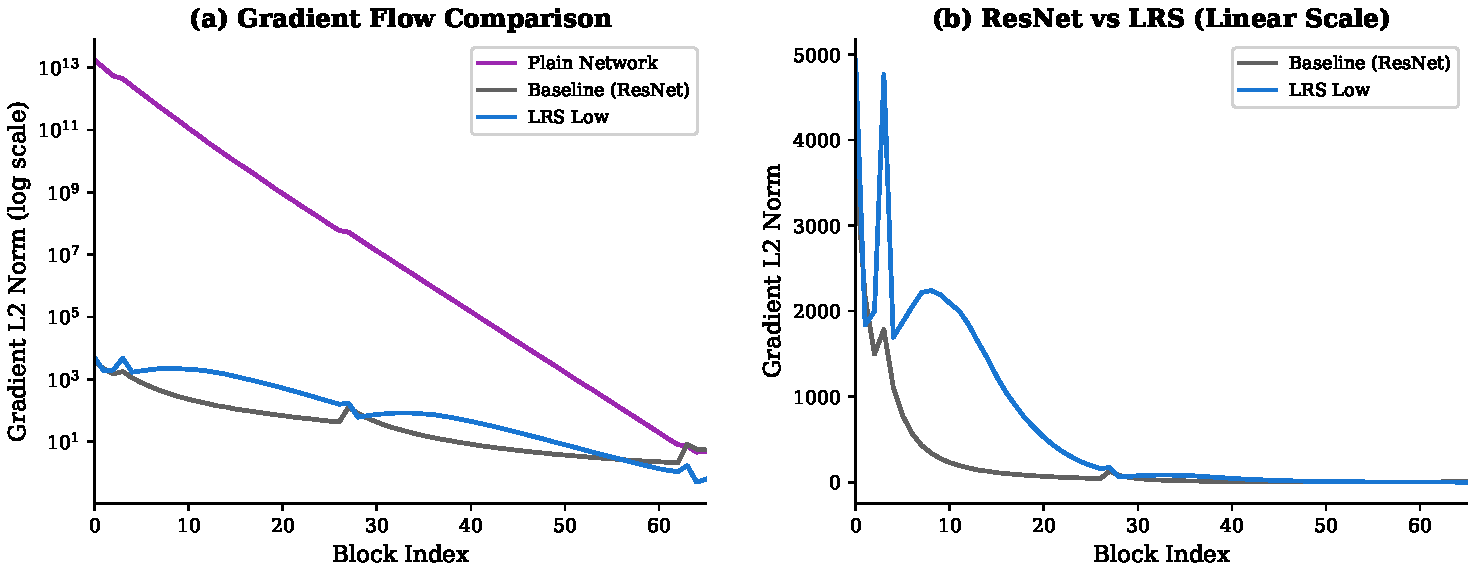
\includegraphics[width=0.95\linewidth]{figures/fig0_gradient_flow.pdf}
    \caption{CIFAR-100, ResNet-200의 초기화 시점 블록별 그래디언트 L2 노름. (a) 스킵 연결이 없는 일반 신경망은 깊이 자율 선택이 불가능하다---초기 블록의 그래디언트가 $>10^{13}$로 폭발한다. 스킵 연결은 그래디언트 분포를 안정화한다. (b--c) LRS를 사용하면 후기 블록 그래디언트가 0에 가깝게 감쇠하며, 이는 신경망의 학습된 선택 $\alpha_i \approx 0$을 반영한다: 그 블록들은 사용되지 않는다.}
    \label{fig:gradient_flow}
\end{figure}

\textbf{기여 사항.}
(1) 우리는 ResNet이 효과적 깊이의 자율 선택에 의해 학습에 성공하며, 스킵 연결이 이를 가능케 한다고 제안한다; LRS가 이를 측정 가능하게 만든다.
(2) 우리는 CIFAR-10/100과 ImageNet의 여러 깊이에 걸쳐 성립하는 깊이--$\alpha$ 스케일링 법칙을 경험적으로 확립한다.
(3) 우리는 가지치기, 항등 초기화 불변성, 초기화 민감도 분석을 통해 측정이 의미적으로 유효함을 검증한다; $\alpha$ 기반 가지치기는 정확도 4.6\% 손실로 FLOPs 54\% 감소를 달성한다.
(4) 우리는 퇴화 문제를 재구성한다: 그것은 해결해야 할 실패가 아니라 신경망이 불필요한 깊이의 사용을 거부하는 현상이다.

% ============================================================
\section{관련 연구}
\label{sec:related}

\subsection{잔차 신경망과 스킵 연결}

ResNet~\cite{he2016deep}은 깊은 신경망의 그래디언트 소실 완화를 위해 스킵 연결을 도입했고, 항등 매핑은 그래디언트 흐름을 더 개선한다~\cite{he2016identity}. Highway Networks~\cite{srivastava2015highway}는 ResNet 이전에 게이트 기반 정보 흐름을 제안했다. De \& Smith~\cite{de2020batch}는 배치 정규화가 표준 ResNet의 잔차를 항등 쪽으로 편향시킨다는 점을 보였고---이는 LRS가 명시적으로 만들지만 \emph{창출}하지는 않는 현상이다.

\subsection{잔차 스케일링 방법}

여러 방법이 잔차 분기를 스케일링한다(표~\ref{tab:comparison}). \textbf{ReZero}~\cite{bachlechner2021rezero}는 잔차 분기에 스칼라 곱셈자 $\alpha = 0$을 초기화한다: $y = x + \alpha F(x)$. \textbf{SkipInit}~\cite{de2020batch}은 배치 정규화를 유지하면서 같은 형식을 적용한다. \textbf{Fixup}~\cite{zhang2019fixup}은 각 블록의 마지막 BN을 0으로 초기화해 시작 시 $F(x) \approx 0$이 되게 한다. \textbf{LayerScale}~\cite{touvron2021going}은 비전 트랜스포머에 채널별 학습 가능 스케일링을 도입한다. 이 모든 방법은 $F(x)$만 스케일링하고 $x$를 가중치 $1$로 유지한다. LRS는 대신 단일 스칼라로 두 분기의 상대적 가중치를 학습하며, 이것이 블록별 사용량 측정의 핵심이다.

\begin{table}[!ht]
\centering
\small
\caption{잔차 스케일링 방법. LRS만이 $F(x)$와 $x$의 상대 비율을 블록별 단일 스칼라로 측정하여 직접적 효과적 깊이 측정을 가능케 한다.}
\label{tab:comparison}
\begin{tabular}{lccc}
\toprule
\textbf{방법} & \textbf{정식화} & \textbf{블록별 측정 가능} & \textbf{핵심 차이} \\
\midrule
ReZero & $y = x + \alpha F(x)$ & $|F(x)|$ 스케일 & $x$ 가중치 1 고정 \\
SkipInit & $y = x + \alpha F(x)$ & $|F(x)|$ 스케일 & $x$ 가중치 1 고정 \\
LayerScale & $y = x + \Lambda F(x)$ & 채널별 $|F(x)|$ & $x$ 가중치 1 고정 \\
Fixup & $y = x + \beta F(x)$ & $|F(x)|$ 스케일 & 마지막 레이어 0 초기화 \\
\textbf{LRS (제안)} & $\mathbf{y = \alpha F(x) + (1{-}\alpha)x}$ & $\mathbf{F(x){:}x}$ \textbf{비율} & \textbf{양쪽 조정} \\
\bottomrule
\end{tabular}
\end{table}

\subsection{Highway Networks와의 비교}

Highway Networks~\cite{srivastava2015highway}는 유사한 볼록 결합 $y = T(x) F(x) + (1{-}T(x)) x$를 $T(x) = \sigma(W_g x + b_g)$와 함께 사용한다. 그러나 차이는 구조적이고 본 분석의 핵심이다. Highway의 변환 게이트 $T(x)$는 \emph{입력 의존적}이다: 모든 입력이 다른 게이트 값을 산출하므로 블록별 사용량을 단일 숫자로 요약할 수 없다. LRS는 대신 \emph{입력 비의존적} 스칼라 $\alpha = \sigma(\theta)$를 사용하여, 블록별 측정을 얻기 위해 의도적으로 입력 의존성을 제거한다. 이는 해석가능성을 위한 방법론적 선택이다: 블록당 단일 $\alpha$는 ``이 블록이 입력을 얼마나 변환하는가''라는 양을 잘 정의된 것으로 만들어, 깊이--$\alpha$ 스케일링 법칙, 블록별 분포 분석, 가지치기 검증을 가능케 한다. Highway 게이트는 입력 분포에 대한 평균을 내야 비교 가능한 스칼라가 산출되며---이는 우리의 설계가 동기로 삼는 해석가능성 자체를 잃게 한다.

\subsection{효과적 깊이와 신경망 잉여성}

Huang \etal~\cite{huang2016deep}은 학습 중 잔차 블록을 무작위로 드롭하는 stochastic depth를 제안하여, 모든 블록이 필요하지 않음을 보였다. lottery ticket 가설~\cite{frankle2019lottery}은 큰 신경망이 전체 신경망의 성능에 필적하는 작은 부분망을 포함한다는 것을 입증했다. 가장 가까운 선행 연구는 Veit \etal~\cite{veit2016residual}로, ResNet을 경로 앙상블로 해석하고 효과적 경로가 명목 깊이보다 훨씬 짧음을 경험적으로 보였다. 그러나 선행 증거는 \emph{간접적}이다: 경로 앙상블 분석은 다양한 길이의 경로를 세고, 절제 연구는 블록을 삭제하고 퇴화를 측정해 중요도를 추론한다. ``블록 $i$가 실제로 얼마나 기여하는가''라는 질문은 추론적으로만 답해진다. LRS는 \emph{직접적이고 블록별이며 정량적인 측정}을 제공한다: 학습된 $\alpha_i$ 값이 \emph{그 자체로} 블록의 기여이며, 사후 분석 없이 관찰 가능하다. 이 직접적 측정 가능성은 (i) 정량적 스케일링 법칙 $\bar{\alpha}(L)$, (ii) 임계값 없는 효과적 깊이 척도 $D_\text{eff} = \sum_i \alpha_i$, (iii) $\alpha < 0.03$에서의 무손실 제거로 검증된 원칙적 가지치기 기준을 가능케 한다.

\subsection{학습된 중요도 가지치기와의 비교}

블록 내 학습 가능 스칼라를 가지치기를 위한 중요도 신호로 사용하는 관련 연구가 있다. Network Slimming~\cite{liu2017slimming}은 배치 정규화의 $\gamma$를 채널별 중요도 점수로 재활용하며, $L_1$ 정규화를 적용해 희소성을 유발한다. 메커니즘은 표면적으로는 유사하지만---학습된 스칼라가 컴포넌트 사용량을 드러낸다는 점---피연산자와 의미는 세 축에서 근본적으로 다르다. \textbf{입도}: Network Slimming은 고정된 깊이 내에서 \emph{채널별} 중요도를 측정한다; LRS는 \emph{블록별} 사용량을 측정하여 신경망 수준의 효과적 깊이 $D_\text{eff}$를 산출한다. \textbf{해석}: $\gamma$는 단일 정규화 특징을 스케일링하며 희소화에 명시적 $L_1$ 압력이 필요하다; $\alpha$는 의미($F{:}x$ 비율)가 본질적인 볼록 결합 가중치이며 별도의 희소성 사전 없이도 작은 $\alpha$가 학습 동역학으로부터 자연 발생한다. \textbf{주장}: Network Slimming은 가지치기 방법이다; LRS는 분석 도구이며, 가지치기 실험은 자율 선택 명제에 대한 \emph{검증}이지 기여 그 자체가 아니다. Channel Pruning~\cite{he2017channel}과 유사한 학습된 중요도 방법들도 Network Slimming의 관점을 공유하며, 우리와는 상보적이다.

% ============================================================
\section{방법}
\label{sec:method}

\subsection{학습 가능한 잔차 스케일링}

우리는 잔차 블록을 식 (\ref{eq:lrs})로 재정의한다. 여기서 $\theta$는 블록당 학습 가능한 스칼라 파라미터이며 $\sigma$는 시그모이드이다. 이 매개변수화는 두 가지 목적을 갖는다. 첫째, $\alpha + (1-\alpha) = 1$이므로 $F(x)$와 $x$의 \emph{상대 비율}이 직접 해석 가능하다: $\alpha = 0.14$는 블록이 변환에 14\%, 항등에 86\%를 할당함을 의미한다. 둘째, 제한된 범위는 수치적 안정성을 보장한다. 이 의미론은 효과적 깊이의 자연스러운 정의를 부여한다: $\alpha \to 0$이면 블록은 사실상 우회되고 ($y \approx x$), $\alpha \to 1$이면 완전한 변환을 수행한다. 신경망의 효과적 깊이는 의미 있는 임계값을 넘는 $\alpha$를 가진 블록의 수이며, $D_\text{eff} = \sum_i \alpha_i$가 임계값 없는 대응물이다.

\subsection{그래디언트 흐름 분석}

LRS 블록의 역전파는 다음을 산출한다:
\begin{equation}
    \frac{\partial \mathcal{L}}{\partial x} = \frac{\partial \mathcal{L}}{\partial y} \left[ (1 - \alpha) + \alpha \cdot F'(x) \right]
    \label{eq:grad}
\end{equation}
그리고 $L$개 블록을 통한 총 그래디언트는 곱이다:
\begin{equation}
    \frac{\partial \mathcal{L}}{\partial x_0} = \frac{\partial \mathcal{L}}{\partial y_L} \cdot \prod_{i=1}^{L} \left[ (1 - \alpha_i) + \alpha_i \cdot F'_i(x_i) \right].
    \label{eq:total_grad}
\end{equation}
이 곱 구조가 깊이--$\alpha$ 관계를 설명한다. $L$개 블록에서 곱이 안정되려면 각 인자가 $1$에 가까워야 한다. $\alpha_i$가 작으면 인자는 $F'_i$와 무관하게 $(1{-}\alpha_i) \approx 1$에 접근하여 그래디언트 안정성을 보장한다. $L$이 증가할수록 곱을 단위 근처에 유지하려면 더 작은 $\alpha_i$ 값이 필요하며, 이는 더 깊은 신경망이 더 작은 $\bar{\alpha}$로 수렴해야 하는 이론적 근거를 제공한다. 반대로 $\alpha_i$가 크면 인자는 $\approx F'_i$가 되어 그래디언트 곱이 일반 신경망의 그것으로 퇴화하며, 소실 또는 폭발 경향을 보인다. 이는 잔차 선호 초기화가 극단적 깊이에서 학습 붕괴를 일으킬 것을 예측한다---섹션~\ref{sec:init_sensitivity}에서 검증된다.

\subsection{초기화 변형}

수렴성과 민감도를 연구하기 위해 우리는 세 가지 초기화 전략을 시험한다(표~\ref{tab:init_variants}). 이들은 탐침 역할을 한다: 최적화 풍경에 단일 분지(basin)가 있다면 셋 다 같은 $\bar{\alpha}$로 수렴할 것이다; 그렇지 않다면 발산이 초기 조건의 역할을 드러낸다.

\begin{table}[!ht]
\centering
\small
\caption{$\alpha$ 초기화에 의한 LRS 변형. 세 시작점은 $\alpha$가 같은 최적점으로 수렴하는지 탐침한다.}
\label{tab:init_variants}
\begin{tabular}{lccc}
\toprule
\textbf{변형} & $\theta_0$ & $\alpha_0$ & \textbf{초기 편향} \\
\midrule
LRS Low  & $-2.0$ & $\approx 0.12$ & 항등 선호 \\
LRS Mid  & $0.0$  & $0.50$         & 균형 \\
LRS High & $+2.0$ & $\approx 0.88$ & 잔차 선호 \\
\bottomrule
\end{tabular}
\end{table}

% ============================================================
\section{실험}
\label{sec:experiments}

\subsection{실험 설정}
\label{sec:setup}

\textbf{데이터셋.} 체계적 분석을 위해 CIFAR-10/100~\cite{krizhevsky2009learning} (10/100 클래스, 50K/10K 학습/시험); 규모 검증을 위해 ImageNet~\cite{russakovsky2015imagenet} (1000 클래스, 1.28M/50K).

\textbf{아키텍처.} 병목(bottleneck) ResNet-50/101/152/200 (16/33/50/66 블록). CIFAR는 $3{\times}3$ stride-1 stem을, ImageNet은 표준 $7{\times}7$ stride-2 + max-pool stem~\cite{he2016deep}을 사용한다.

\textbf{학습.} CIFAR: SGD with 모멘텀 0.9, 가중치 감쇠 $10^{-4}$; 초기 LR $0.1$, 코사인 어닐링~\cite{loshchilov2017sgdr}; 5에포크 선형 워밍업; 100 에포크. 배치 크기는 깊이 의존적이다(GPU 메모리로 인해 깊이 $50, 101, 152, 200$에서 각각 $128, 64, 32, 32$). ImageNet: 동일 최적화기, LR $0.2$, 배치 크기 $512$ (고정), $60$ 에포크, $5$-에포크 워밍업. 모든 CIFAR 실험은 시드 3개 (42, 123, 456)를 사용하고 평균 $\pm$ 표준편차를 보고하며, ImageNet은 시드 1개를 사용한다. CIFAR 깊이별 배치 크기 변동은 알려진 혼동 요인이다; 그러나 \emph{고정} 배치 크기 $512$의 ImageNet도 CIFAR-100과 동일한 $\bar{\alpha}$ 스케일링 기울기($d50 \to d101$에서 $0.303 \to 0.166$, 45\% 감소 vs.\ $0.342 \to 0.183$, 46\% 감소)를 보여, 배치 크기가 깊이--$\bar{\alpha}$ 관계의 주된 원인이 아님을 시사한다.

\textbf{모델.} 다섯 가지 핵심 변형: Baseline (표준 ResNet), LRS Low/Mid/High ($\alpha_0 \in \{0.12, 0.5, 0.88\}$), ReZero. 방법 비교를 위해 SkipInit, Fixup, LayerScale도 추가 평가한다.

\subsection{깊이--$\alpha$ 스케일링 법칙}
\label{sec:alpha_convergence}

먼저 중심 관찰을 측정한다: 깊이에 따라 신경망의 선호 $\bar{\alpha}$는 어떻게 변하는가? 표~\ref{tab:depth_alpha}은 세 초기화 변형에 대한 CIFAR-100의 수렴 $\bar{\alpha}$를 보고한다 (시드 3개 평균).

\begin{table}[!ht]
\centering
\small
\caption{CIFAR-100의 깊이별 평균 수렴 $\bar{\alpha}$ (시드 3개 평균). Low와 Mid는 유사한 최종값으로 수렴; High는 극단적 깊이에서 발산.}
\label{tab:depth_alpha}
\begin{tabular}{lcccc}
\toprule
\textbf{깊이} & \textbf{블록 수} & \textbf{LRS Low} & \textbf{LRS Mid} & \textbf{LRS High} \\
\midrule
50  & 16 & 0.34 & 0.35 & 0.36 \\
101 & 33 & 0.18 & 0.20 & 0.21 \\
152 & 50 & 0.13 & 0.15 & 0.23 \\
200 & 66 & 0.11 & 0.13 & 0.28 \\
\bottomrule
\end{tabular}
\end{table}

몇 가지 관찰이 도출된다. (i) \textbf{깊이에 따른 단조 감소.} 수렴 $\bar{\alpha}$는 LRS Low에서 $0.34$(깊이 50)에서 $0.11$(깊이 200)로 감소한다---각 블록의 기여는 블록이 더 추가될수록 줄어든다. (ii) \textbf{초기화 간 부분 수렴.} 깊이 50에서는 세 변형이 비슷한 값($0.34$--$0.36$)으로 수렴한다. 깊이 200에서는 High 변형이 $0.28$에 멈춰 Low/Mid의 $0.11$--$0.13$ 범위보다 훨씬 위에 있으며, 성능도 심각하게 저하된다(섹션~\ref{sec:init_sensitivity}). (iii) \textbf{데이터셋 독립성.} CIFAR-10이 각 깊이에서 거의 동일한 $\bar{\alpha}$를 산출하여 데이터 의존이 아닌 아키텍처적 특성을 시사한다.

\textbf{규모에서의 검증.} 법칙이 CIFAR 너머로 일반화되는지 확인하기 위해 두 깊이에서 ImageNet의 $\bar{\alpha}$를 측정한다 (그림~\ref{fig:depth_alpha}). ResNet-50은 $\bar{\alpha} = 0.303$, ResNet-101은 $\bar{\alpha} = 0.166$을 산출한다. 두 값 모두 CIFAR-100의 동일 깊이 값($0.342, 0.183$)을 가깝게 추종하며 동일한 스케일링 추세를 따른다. ImageNet은 CIFAR보다 학습 샘플이 $\sim$25$\times$, 클래스가 10$\times$, 입력 해상도가 7$\times$ 크다; 이 격차에 걸쳐 $\alpha$ 패턴이 지속된다는 사실은 단순한 데이터셋 크기 설명을 배제한다.

비록 ImageNet은 compute 제약으로 시드 1개를 사용하지만, CIFAR 스케일링 법칙은 시드 간 분산이 매우 작다: 깊이 $(50, 101, 152, 200)$에서 $\bar{\alpha}$ 표준편차는 $(0.0007, 0.0005, 0.0012, 0.0002)$로 모두 평균의 $1\%$ 미만이다. 일치 깊이에서의 ImageNet--CIFAR-100 격차는 $d50$에서 $0.342{-}0.303 = 0.039$, $d101$에서 $0.183{-}0.166 = 0.017$로, 둘 다 CIFAR 시드 노이즈 척도의 20--80$\times$ 더 크다. 작지만 체계적인 데이터셋 시프트이며 단조성은 보존된다. ImageNet의 $d50 \to d101$ $\bar{\alpha}$ 비율은 $0.303/0.166 = 1.83$로, CIFAR-100의 비율 $0.342/0.183 = 1.87$과 본질적으로 일치한다; 스케일링 법칙의 기울기가 데이터셋 격차에 걸쳐 보존된다. 이 격차-대-노이즈 비율에서 두 깊이에 걸쳐 동일한 감소 추세를 만드는 통계적 우연은 비현실적이다.

\begin{figure}[!ht]
    \centering
    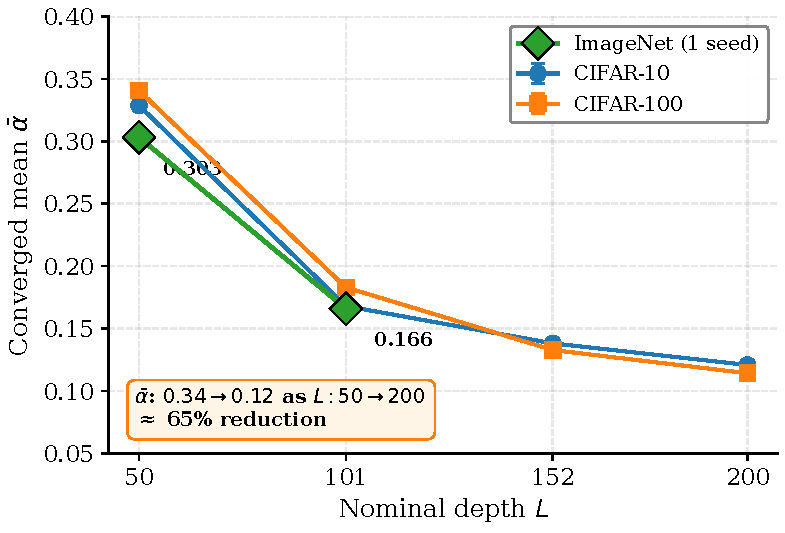
\includegraphics[width=0.72\linewidth]{figures/fig_depth_alpha_v2.pdf}
    \caption{깊이--$\bar{\alpha}$ 스케일링 법칙. 평균 수렴 $\bar{\alpha}$는 CIFAR-10, CIFAR-100, ImageNet에서 명목 깊이 $L$에 따라 단조 감소한다. 깊이가 $50 \to 200$으로 증가함에 따라 ResNet은 잔차 기여의 약 65\%를 자율적으로 억제한다. 오차 막대: 시드 3개에 대한 $\pm 1$ 표준편차 (CIFAR); ImageNet은 시드 1개 사용.}
    \label{fig:depth_alpha}
\end{figure}

\subsection{블록별 $\alpha$ 분포}
\label{sec:perblock}

평균은 구조를 숨긴다. 그림~\ref{fig:perblock_alpha}은 200층 신경망(66 블록, LRS Low, CIFAR-100)의 블록별 $\alpha$를 보여준다. 두 패턴이 드러난다: \textbf{다운샘플링 블록은 높은 $\alpha$를 갖는다} (0.42--0.96); \textbf{일반 블록은 낮은 $\alpha$를 갖는다} (0.06--0.15)이며 스테이지 끝으로 갈수록 점진적으로 감소한다. 신경망은 각 스테이지를 ``하나의 필수 변환(다운샘플링) 뒤에 점진적으로 무시 가능한 정제들''로 취급한다.

\begin{figure}[!ht]
    \centering
    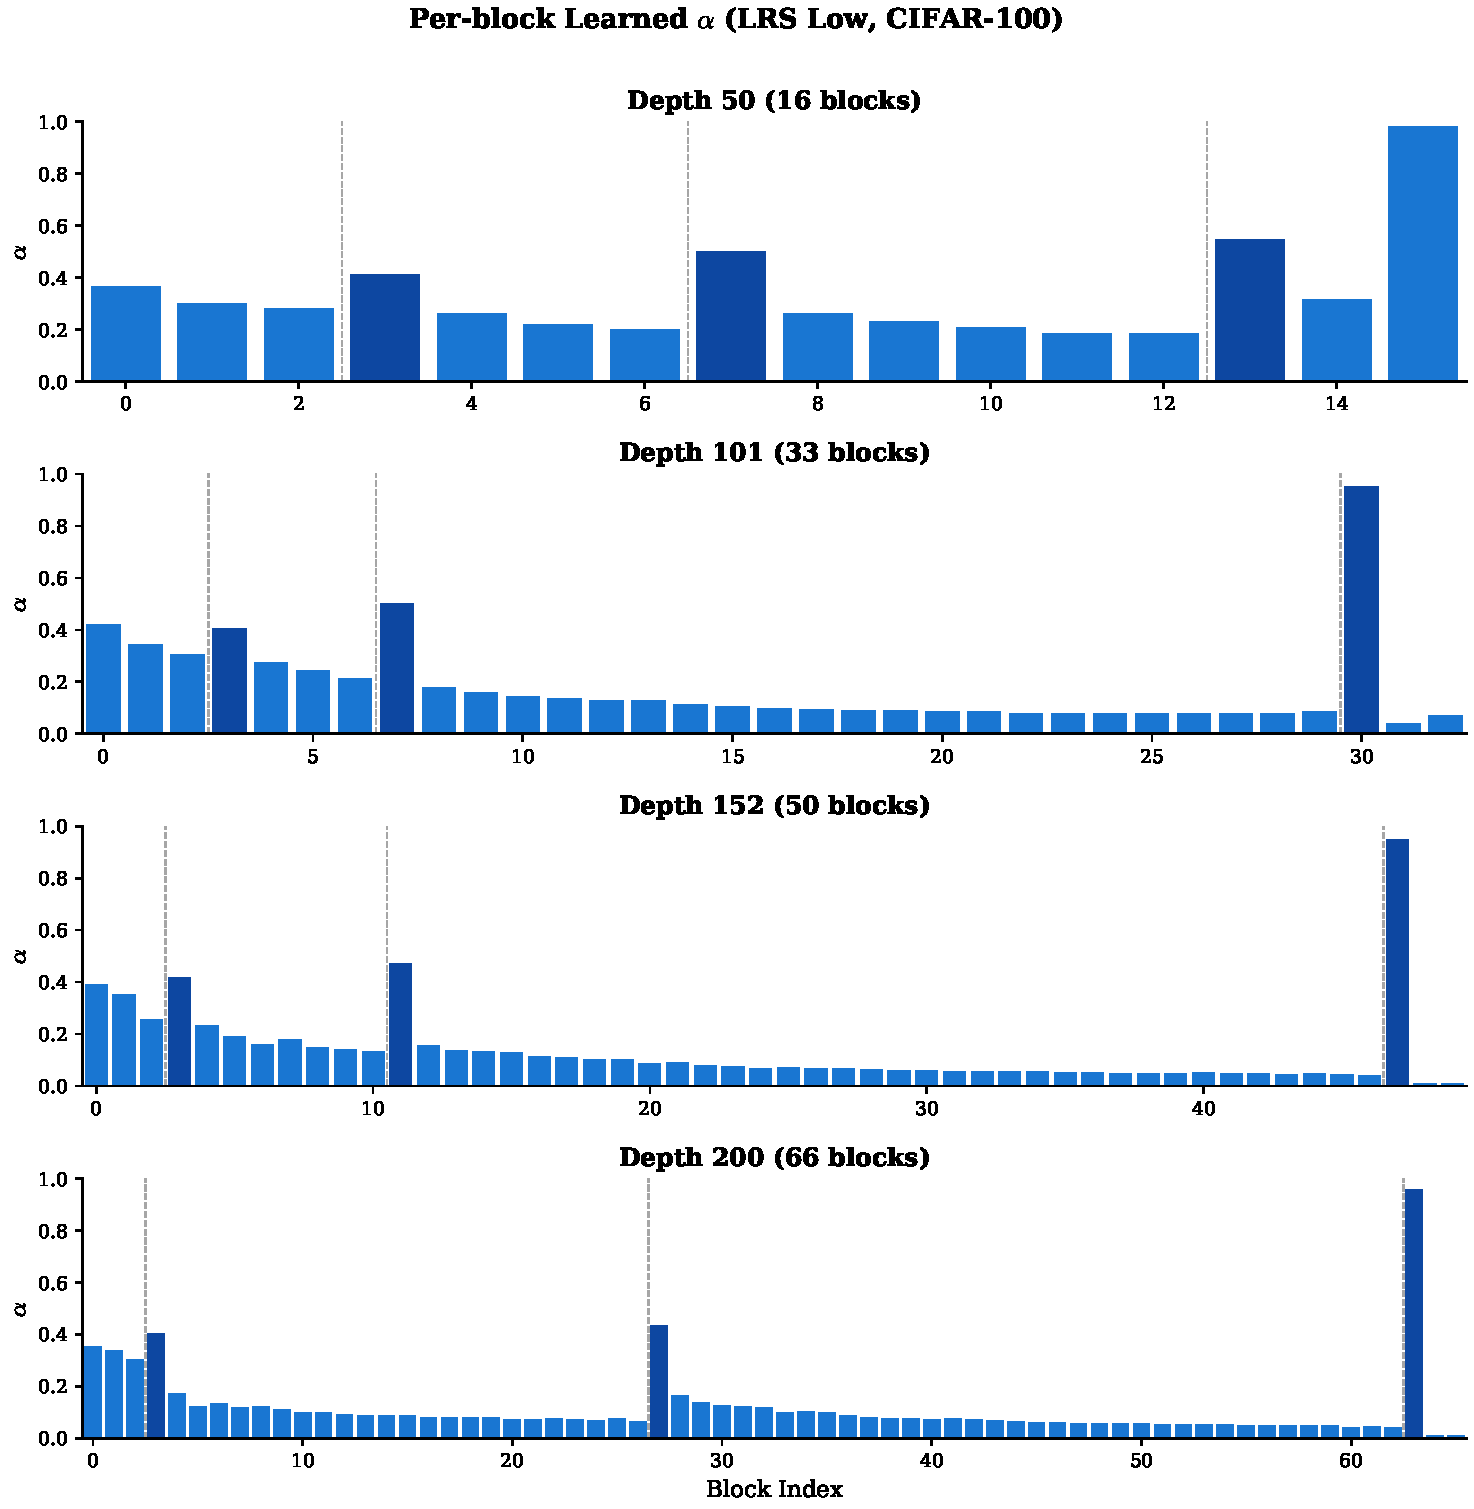
\includegraphics[width=0.85\linewidth]{figures/fig4_perblock_alpha.pdf}
    \caption{CIFAR-100, ResNet-200의 블록별 $\alpha$. 스테이지 경계 (다운샘플링 블록)는 높은 $\alpha$를 유지하고, 스테이지 내 블록은 거의 0에 수렴한다.}
    \label{fig:perblock_alpha}
\end{figure}

\subsection{효과적 깊이 정량화}
\label{sec:effective_depth}

$\alpha > 0.3$을 ``활성 블록''의 임계값으로 사용하면, 200층 신경망의 66 블록 중 5--6개만 자격을 갖는다---효과적 깊이는 명목의 $\sim$8\%이다. 임계값 의존성을 피하기 위해 임계값 없는 척도 $D_\text{eff} = \sum_i \alpha_i$도 보고한다(표~\ref{tab:deff}): 블록 수가 4배 증가($16 \to 66$)해도 $D_\text{eff}$는 단 40\%만 증가한다 ($5.4 \to 7.5$). 블록별 분해를 보면 스테이지 내 $\bar{\alpha}$는 $[0.06, 0.15]$ (거의 항등)에 머물고, 다운샘플링 블록 $\bar{\alpha}$는 $[0.42, 0.96]$ (활성 변환)에 머문다.

\begin{table}[!ht]
\centering
\small
\caption{CIFAR-100, LRS Low의 임계값 없는 효과적 깊이 $D_\text{eff} = \sum_i \alpha_i$. 명목 깊이가 4배 늘어도 $D_\text{eff}$는 단 1.4배 늘어난다, 추가된 블록 대부분이 사용되지 않음을 확인.}
\label{tab:deff}
\begin{tabular}{lcccc}
\toprule
\textbf{깊이} & \textbf{블록 수} ($N$) & $D_\text{eff} = \sum \alpha_i$ & $D_\text{eff}/N$ & \textbf{활성} ($\alpha{>}0.3$) \\
\midrule
50  & 16 & 5.4 & 34.0\% & 6--7 \\
101 & 33 & 6.0 & 18.3\% & 6 \\
152 & 50 & 6.7 & 13.3\% & 5--6 \\
200 & 66 & 7.5 & 11.4\% & 5--6 \\
\bottomrule
\end{tabular}
\end{table}

\subsection{초기화 민감도}
\label{sec:init_sensitivity}

세 초기화는 깊이에 따른 학습 안정성의 극적인 차이를 드러낸다 (표~\ref{tab:cifar10}, \ref{tab:cifar100}). LRS Low는 모든 깊이에서 baseline과 동등하거나 능가하며 낮은 분산을 보인다. LRS Mid는 깊이 200에서 저하된다. LRS High는 점진적 저하를 보이고 결국 처참히 실패한다(CIFAR-100: $37.50 \pm 29.20\%$). 메커니즘은 그래디언트 보존이다(식 \ref{eq:total_grad}): $\alpha_0 = 0.88$이면 66개 블록에서 항등 기저선은 $0.12^{66} \approx 0$이 되어 빠른 $\alpha$ 조정 없이는 학습 불가능한데, 그 조정 자체도 그래디언트가 필요하다.

\begin{table}[!ht]
\centering
\small
\caption{CIFAR-10 시험 정확도 (\%, 시드 3개 평균 $\pm$ 표준편차). LRS High는 깊이 200에서 붕괴.}
\label{tab:cifar10}
\begin{tabular}{lccccc}
\toprule
\textbf{깊이} & \textbf{Baseline} & \textbf{LRS Low} & \textbf{LRS Mid} & \textbf{LRS High} & \textbf{ReZero} \\
\midrule
50  & 94.53$\pm$0.14 & \textbf{94.83}$\pm$0.13 & 94.77$\pm$0.03 & 94.27$\pm$0.17 & 94.60$\pm$0.28 \\
101 & 95.37$\pm$0.11 & \textbf{95.44}$\pm$0.12 & 95.15$\pm$0.11 & 94.28$\pm$0.29 & 95.38$\pm$0.21 \\
152 & 95.95$\pm$0.06 & 95.73$\pm$0.10 & 95.60$\pm$0.15 & 93.78$\pm$0.87 & \textbf{95.99}$\pm$0.06 \\
200 & 95.98$\pm$0.15 & \textbf{96.10}$\pm$0.12 & 94.36$\pm$0.92 & 67.25$\pm$43.65 & 96.02$\pm$0.16 \\
\bottomrule
\end{tabular}
\end{table}

\begin{table}[!ht]
\centering
\small
\caption{CIFAR-100 시험 정확도 (\%, 시드 3개 평균 $\pm$ 표준편차). LRS High는 처참히 실패.}
\label{tab:cifar100}
\begin{tabular}{lccccc}
\toprule
\textbf{깊이} & \textbf{Baseline} & \textbf{LRS Low} & \textbf{LRS Mid} & \textbf{LRS High} & \textbf{ReZero} \\
\midrule
50  & 77.18$\pm$0.36 & 77.02$\pm$0.20 & 76.72$\pm$0.40 & 75.22$\pm$0.45 & 76.12$\pm$0.09 \\
101 & \textbf{79.29}$\pm$0.23 & 78.85$\pm$0.14 & 78.34$\pm$0.19 & 75.16$\pm$1.69 & 78.04$\pm$0.48 \\
152 & \textbf{80.42}$\pm$0.22 & 80.28$\pm$0.38 & 78.57$\pm$0.60 & 71.66$\pm$3.40 & 79.72$\pm$0.10 \\
200 & \textbf{80.72}$\pm$0.17 & 80.65$\pm$0.01 & 76.07$\pm$1.59 & 37.50$\pm$29.20 & 80.14$\pm$0.17 \\
\bottomrule
\end{tabular}
\end{table}

\subsection{본질적 vs.\ 인위적 산물: 항등 초기화 시험}
\label{sec:identity_init}

자연스러운 우려: 낮은 효과적 깊이가 무작위로 초기화된 잔차 분기의 산물 아닌가? 우리는 잔차 분기를 항등 변환으로 초기화하여 이를 시험한다(HybridA: 레이어 3, 4에 대해 항등 초기화; Full Identity: 모든 레이어). CIFAR-100 결과(표~\ref{tab:identity_init}): full identity init은 처참히 실패한다 (깊이 200에서 12.98\%), 신경망이 깰 수 없는 대칭으로 인해. 부분 항등 초기화 + LRS는 최고 정확도를 달성한다 (81.14\%). \emph{결정적으로}, 학습된 $\bar{\alpha}$는 무작위와 항등 초기화 사이에서 거의 동일하다 ($0.114$ vs.\ $0.118$, 66 블록 중 활성 5 vs.\ 6). 신경망은 잔차 분기가 어디에서 시작하든 같은 효과적 깊이로 수렴한다---초기화가 낮은 효과적 깊이의 원인이라는 가설을 배제한다.

\begin{table}[!ht]
\centering
\small
\caption{항등 초기화 분석 (CIFAR-100, 시드 3개 평균 $\pm$ 표준편차). 효과적 깊이는 잔차 분기 초기화에 불변.}
\label{tab:identity_init}
\begin{tabular}{lcccc}
\toprule
\textbf{모델} & \textbf{d152 (\%)} & \textbf{d200 (\%)} & $\mathbf{\bar{\alpha}}$ \textbf{(d200)} & \textbf{활성 / 66} \\
\midrule
Baseline (He init) & 80.42$\pm$0.18 & 80.72$\pm$0.13 & --- & --- \\
LRS Low + He init & 80.28$\pm$0.31 & 80.65$\pm$0.01 & 0.114 & 5 \\
HybridA (Identity L3,4) & 80.02$\pm$0.26 & 80.40$\pm$0.17 & --- & --- \\
LRS Low + HybridA & \textbf{80.72}$\pm$0.29 & \textbf{81.14}$\pm$0.18 & 0.118 & 6 \\
ResNet (Full Identity) & 13.41$\pm$0.41 & 12.98$\pm$0.16 & --- & --- \\
\bottomrule
\end{tabular}
\end{table}

\subsection{고정 vs.\ 학습된 $\alpha$}
\label{sec:fixed_alpha}

\emph{학습}이 본질적임을 검증하기 위해 깊이 152에서 고정 $\alpha$ 변형과 비교한다 (표~\ref{tab:fixed_alpha}). 두 가지 발견. (i) 고정 $\alpha = 0.5$는 단 $44.19\%$인데, 이는 정식화 $0.5 F(x) + 0.5 x$가 표준 ResNet의 $F(x) + x$와 달리 두 분기를 균일하게 절반화하기 때문이다. 우리는 이를 sweep의 완전성을 위해 포함하지만, 그 결과 저하는 크기(magnitude)의 역할과 할당의 역할을 혼동하므로 핵심 비교로 읽어서는 안 된다. (ii) 관련 비교는 학습된 평균에 가까운 고정 $\alpha = 0.1$로, 학습된 LRS보다 여전히 $0.47\%$ 낮다. 작지만 이 격차는 학습된 LRS가 블록별 이질성을 활용함과 일관된다: 다운샘플링 블록은 $\alpha \in [0.42, 0.96]$을 유지하고 스테이지 내 블록은 $\alpha \in [0.06, 0.15]$에 안정화된다 (섹션~\ref{sec:perblock}). 균일 상수는 이 구조를 포착할 수 없다.

\begin{table}[!ht]
\centering
\small
\caption{CIFAR-100, 깊이 152의 고정 vs.\ 학습된 $\alpha$. 학습된 블록별 구조가 본질적.}
\label{tab:fixed_alpha}
\begin{tabular}{lcc}
\toprule
\textbf{구성} & \textbf{정확도 (\%)} & \textbf{비고} \\
\midrule
학습 (LRS Low) & \textbf{80.28} & 블록별 $\alpha$, 평균 $\approx 0.13$ \\
고정 $\alpha = 0.1$ & 79.81 & 학습 평균에 근접 \\
고정 $\alpha = 0.3$ & 67.94 & 적당한 변환 \\
고정 $\alpha = 0.5$ & 44.19 & 두 분기를 절반화 \\
고정 $\alpha = 0.7$ & 20.62 & 잔차 선호 \\
\midrule
Baseline ($F(x){+}x$) & 80.42 & LRS 없음 \\
\bottomrule
\end{tabular}
\end{table}

\subsection{$\alpha$ 기반 가지치기와 효율성}
\label{sec:pruning}

만약 $\alpha_i$가 진정으로 블록 사용량을 보고한다면, 매우 낮은 $\alpha$의 블록은 해 없이 제거 가능해야 한다---명제의 직접적 경험적 시험이다. 우리는 $\alpha < \tau$인 블록을 다양한 임계값에 대해 가지치기하여 항등으로 대체하고, 정확도, FLOPs, 추론 지연을 측정한다 (NVIDIA A100 GPU, 배치 크기 1).

표~\ref{tab:pruning}은 ResNet-200/CIFAR-100의 결과를 보고한다. 세 가지 발견:

\begin{table}[!ht]
\centering
\small
\caption{ResNet-200/CIFAR-100의 $\alpha$ 기반 가지치기. 10 에포크 미세 조정으로 정확도 유지; FLOPs와 지연은 실제 단축회로 순전파로 측정.}
\label{tab:pruning}
\begin{tabular}{lcccccc}
\toprule
\textbf{임계값} & \textbf{제거} & \textbf{Acc(미조정)} & \textbf{Acc(+조정)} & $\mathbf{\Delta}$\textbf{Acc} & \textbf{FLOPs} & \textbf{지연} \\
\midrule
없음 (원본) & 0 / 66 & 80.54\% & --- & --- & 100.0\% & 100.0\% \\
$\alpha < 0.03$ & 2 / 66 & 80.54\% & \textbf{80.55\%} & \textbf{$+$0.01} & 97.1\% & 97.7\% \\
$\alpha < 0.05$ & 10 / 66 & 73.88\% & 79.65\% & $-$0.89 & 85.4\% & 86.1\% \\
$\alpha < 0.08$ & 37 / 66 & 3.97\% & 75.91\% & $-$4.63 & \textbf{45.8\%} & \textbf{48.5\%} \\
$\alpha < 0.10$ & 48 / 66 & 3.13\% & 74.74\% & $-$5.80 & 29.7\% & 32.3\% \\
$\alpha < 0.15$ & 58 / 66 & 3.63\% & 72.63\% & $-$7.91 & 15.0\% & 18.0\% \\
\bottomrule
\end{tabular}
\end{table}

\textbf{(a)~$\alpha < 0.03$에서 무손실 가지치기.} 2개 블록 (12 conv/BN 레이어)을 \emph{재학습 없이도} \emph{정확도 손실 없이} 제거 가능하다. 이는 직접적 의미론적 검증이다: 신경망이 $\alpha \approx 0$로 라벨링한 블록은 진정 아무것도 기여하지 않는다.

\textbf{(b)~실용적 효율성 이득.} $\alpha < 0.08$에서 56\%의 블록을 제거하여 FLOPs 54\% 감소, 지연 52\% 감소를 4.6\% 정확도 비용에 (미세 조정 후) 달성한다---강력한 효율성-정확도 거래. $\alpha < 0.10$(73\% 가지치기)에서 신경망은 원본 FLOPs의 단 30\%로 $74.74\%$ 정확도를 유지한다.

\textbf{(c)~자율 선택 vs.\ 최소 충분 깊이.} 미세 조정 없이 $\alpha < 0.08$인 블록을 제거하면 정확도가 $3.97\%$로 붕괴하지만, 10 에포크 미세 조정으로 $75.91\%$로 회복한다. 언뜻 보면 ``5--6개 본질 블록'' 주장과 모순돼 보일 수 있다. 그렇지 않다. $\alpha_i$ 값은 각 블록의 \emph{원본 학습 하에서의 학습된 할당}을 측정한다---신경망이 \emph{사용하기로 선택한} 블록을 식별할 뿐, \emph{유일하게 그 역할을 수행 가능한} 블록을 식별하는 것이 아니다. 5--6개 활성 블록은 \emph{학습된 구성 조건부}로 본질적이다: 미세 조정 없이 제거하면 정확도가 $3.97\%$로 붕괴한다. 미세 조정을 통한 회복은 신경망의 \emph{용량 예비(capacity reserve)}라는 별개의 속성이다: 60개의 휴면 블록은 각자가 거의 항등이지만, 강제로 사용되면 누락된 연산을 집합적으로 재학습할 수 있다. 자율 선택은 따라서 \emph{학습된} 효과적 깊이에 대한 진술이며 \emph{최소 충분} 깊이에 대한 진술이 아니다---그 둘 사이의 격차가 정확히 스킵 연결이 잠재 용량으로 보존하는 ``예비''다.

그림~\ref{fig:pruning}이 정확도-효율성 거래를 시각화한다.

\begin{figure}[!ht]
    \centering
    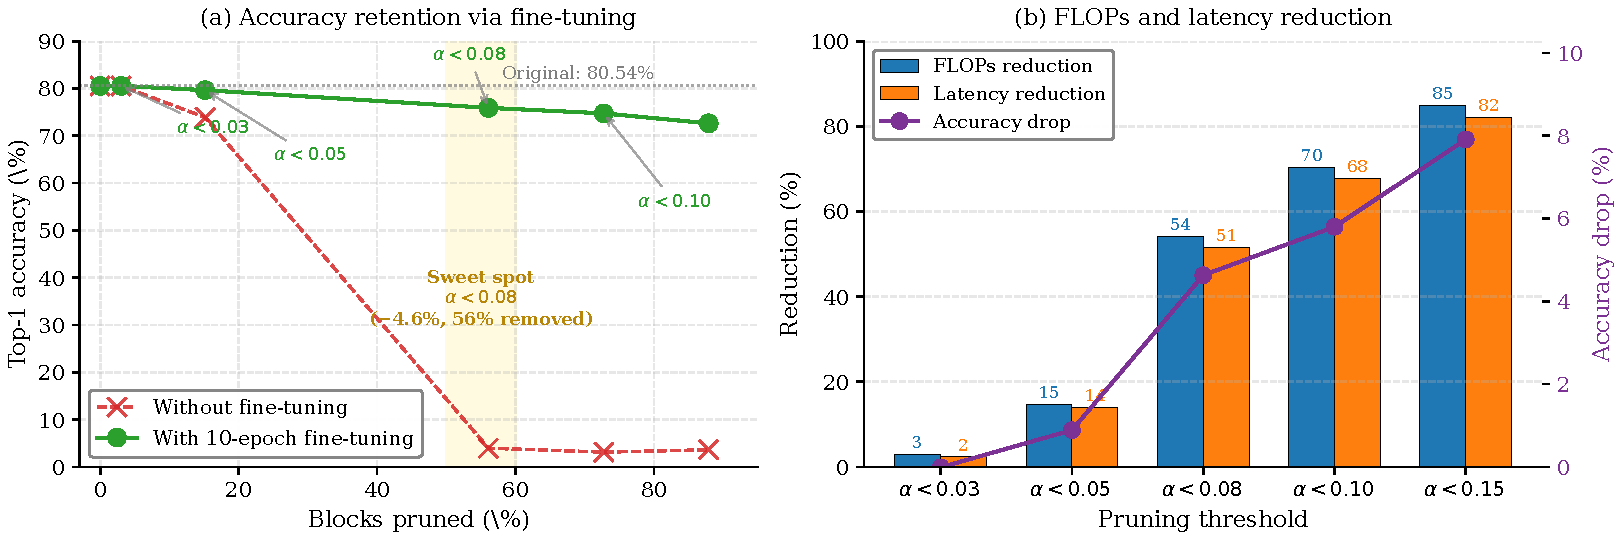
\includegraphics[width=0.88\linewidth]{figures/fig_pruning_efficiency.pdf}
    \caption{ResNet-200/CIFAR-100의 $\alpha$ 기반 가지치기. (a) 미세 조정이 모든 임계값에서 정확도를 회복; 4.6\% 손실로 sweet spot은 $\alpha < 0.08$. (b) $\alpha < 0.08$ 가지치기는 FLOPs 56\%, 추론 지연 51\%를 제거하여 자율 선택된 낮은 $\alpha$ 블록이 기능적으로 거의 항등임을 입증.}
    \label{fig:pruning}
\end{figure}

\subsection{기존 방법과의 비교}
\label{sec:comparison_methods}

CIFAR-100, 깊이 152에서 LRS를 잔차 스케일링 기준선과 비교한다 (표~\ref{tab:method_comparison}, 시드 3개 평균). 모든 방법이 $0.84\%$ 대역 안에 들어간다. 성능 유사성은 예상된 것이다---이는 방법 논문이 아니다. LRS는 블록별 해석 가능성 제공이라는 점에서 차별화된다(표~\ref{tab:comparison}), 정확도 비용 없이.

\begin{table}[!ht]
\centering
\small
\caption{CIFAR-100, 깊이 152의 잔차 스케일링 방법들 (시드 3개 평균). 방법들은 유사하게 수행; LRS만 블록별 측정 제공.}
\label{tab:method_comparison}
\begin{tabular}{lc}
\toprule
\textbf{방법} & \textbf{정확도 (\%)} \\
\midrule
LayerScale & \textbf{80.56} \\
Baseline & 80.42 \\
LRS Low & 80.28 \\
Fixup & 79.79 \\
SkipInit / ReZero & 79.72 \\
\bottomrule
\end{tabular}
\end{table}

% ============================================================
\section{토의}
\label{sec:discussion}

\subsection{ResNet은 자신의 깊이를 자율 선택한다}

중심 발견은 딥 ResNet이 자신의 전체 깊이를 사용하지 않는다는 것이다. 200층 신경망은 변환을 5--6개 블록---주로 스테이지 경계---에 집중시키고 나머지 60개를 거의 항등으로 축소한다. 이는 LRS 측정의 산물이 아니다: 항등 초기화가 같은 결과를 산출하고, 가지치기 검증이 $\alpha < 0.03$ 블록이 진정 아무것도 기여하지 않음을 확인한다.

통상적 견해는 스킵 연결이 깊은 신경망의 그래디언트 흐름을 가능케 해 퇴화 문제를 해결한다는 것이다. 우리의 그래디언트 분석(그림~\ref{fig:gradient_flow})은 그래디언트 안정화를 확인한다. 그러나 LRS는 신경망이 이 안정성을 깊은 연산을 활용하는 데가 아니라 대부분의 블록을 \emph{우회}하는 데 사용함을 드러낸다. 재해석: 퇴화는 해결해야 할 문제가 아니라 신경망이 자신의 최적 깊이를 선택한 자연스러운 결과다. 스킵 연결은 블록이 그래디언트 흐름을 방해하지 않고 거의 항등으로 작동할 수 있게 함으로써 이 자율 선택의 \emph{메커니즘}을 제공한다.

이는 unrolled iterative estimation 견해~\cite{greff2017highway}와 경로 앙상블 해석~\cite{veit2016residual}과 공명한다. 우리의 기여는 경로나 절제로부터 추론하는 대신 $\alpha$를 통해 자율 선택을 직접 관찰 가능하게 만든다는 것이다.

\textbf{Stochastic Depth와의 관계.} Stochastic Depth~\cite{huang2016deep}는 학습 중 블록을 무작위로 드롭해도 정확도가 유지됨을 입증한다. 우리의 발견은 그 반대이자 상보적이다: 연속적인 노브가 주어지면, 신경망 자체가 Stochastic Depth가 무해하게 무작위 드롭할 수 있는 같은 블록에 대해 \emph{결정론적} 거의 항등으로 수렴한다. 두 가지는 같은 현상---스테이지 내 잉여성---을 반대 방향(입력 측 노이즈 vs.\ 학습된 가중치)에서 측정하며, 그들의 일치는 상호 증거이다. 미세 조정 회복 하에 우리가 관찰한 분산 잉여성(섹션~\ref{sec:pruning})은 정확히 무작위 드롭을 가능케 하는 것이다: 블록은 개별적으로 대체 불가능하지 않지만, 표준 학습 하에서 신경망은 활성 역할을 작은 부분집합에 집합적으로 할당한다.

\subsection{다운샘플링 블록의 역할}
\label{sec:downsampling_role}

블록별 분석은 다운샘플링 블록이 높은 $\alpha$(0.42--0.96)를 유지하고 스테이지 내 블록은 $\alpha < 0.15$로 수렴함을 보여준다. 이는 많은 효율적 아키텍처에 암묵적으로 있는 설계 원리를 뒷받침한다: \emph{스테이지 수(따라서 다운샘플링 연산 수)가 스테이지당 총 블록 수보다 중요하다.} 세 갈래의 선행 연구가 이와 일치한다. MobileNet~\cite{howard2017mobilenets}과 EfficientNet~\cite{tan2019efficientnet}은 얕은 스테이지당 블록 수로 강력한 정확도를 달성한다. Stochastic Depth~\cite{huang2016deep}는 스테이지 내 블록을 드롭하는 것이 스테이지-전환 블록을 드롭하는 것보다 덜 해를 미친다는 사실을 발견했다. NAS 문헌~\cite{tan2019efficientnet}은 일관되게 스테이지 전환에 더 많은 채널을 할당하지 추가 스테이지 내 레이어에 할당하지 않는다. LRS는 \emph{왜} 그런지 설명한다: 이러한 방법들이 덜 강조하는 스테이지 내 블록이 정확히 우리의 $\alpha$ 측정이 거의 항등으로 표시하는 블록이다.

\subsection{표준 ResNet이 왜 여전히 잘 작동하는가}

최적 $\alpha$가 0.5보다 훨씬 작다면, 왜 표준 ResNet(암묵적 $\alpha = 0.5$)이 잘 수행되는가? 표준 ResNet은 $y = F(x) + x$를 사용하며, $\|F(x)\|/\|x\|$를 제약하지 않는다. 배치 정규화와 가중치 크기 조정을 통해, 신경망은 명시적 $\alpha$ 없이도 작은 비율을 효과적으로 달성할 수 있다---De \& Smith~\cite{de2020batch}가 독립적으로 확립한 현상이다. LRS는 이 암묵적 비율을 관찰 가능하게 만들고 정량화한다.

\subsection{실용적 함의}
\label{sec:practical_implications}

우리의 발견은 세 가지 실행 가능한 지침으로 번역된다. \textbf{(1) $\alpha$ 기반 가지치기}는 학습 부산물로 산출되는 자동 블록 중요도 기준을 제공한다---일회성 워크플로(LRS로 한 번 학습, $\alpha$ 임계화, $\sim$10 에포크 미세 조정)로 4.6\% 정확도 비용에 54\% FLOPs / 52\% 지연 감소를 산출한다. \textbf{(2) 항등 선호 초기화} ($\alpha_0 \leq 0.12$, $\theta_0 \leq -2$)는 극단적 깊이에서 필수다---잔차 선호 초기화는 학습을 적극적으로 불안정화한다. \textbf{(3) 아키텍처 설계}: 이질적 $\alpha$ 분포는 스테이지 내가 아닌 스테이지 경계에 용량을 할당하는 것을 정당화하며, NAS 절차는 과도하게 깊은 스테이지 내 구성에 대해 $\alpha$ 통계를 정규화기로 사용할 수 있다.

\subsection{한계}

\textbf{ImageNet 규모.} 우리는 ImageNet 깊이 50과 101에서 시드 1개로 스케일링 법칙을 검증한다; 더 깊은 모델과 추가 시드는 주장을 강화할 것이다. CIFAR 시드 노이즈 바닥(평균의 $<1\%$)과 20--80$\times$ 더 큰 ImageNet-CIFAR 격차는 시드 사고에 반대하지만, ImageNet 내부 노이즈는 직접 특성화되지 않았다. \textbf{측정 편향.} LRS는 블록당 하나의 파라미터를 추가한다; 항등 초기화 실험(섹션~\ref{sec:identity_init})은 출발점과 무관한 수렴 $\bar{\alpha}$를 보여 본질적 수렴을 주장한다. \textbf{아키텍처 범위.} 분석은 병목 ResNet에 국한되며, basic 블록과 비전 트랜스포머는 다루지 않는다. \textbf{임계값 의존성.} ``활성 블록'' 임계값 $\alpha > 0.3$은 자의적이며, 임계값 없는 $D_\text{eff} = \sum_i \alpha_i$로 해결된다.

% ============================================================
\section{결론}
\label{sec:conclusion}

우리는 왜 딥 ResNet이 학습에 성공하는가에 대한 구체적 답을 제안하고 경험적으로 뒷받침했다: 그들은 명목 깊이보다 훨씬 작은 효과적 깊이를 자율적으로 선택하며, 스킵 연결은 이 자율 선택을 가능케 하는 구조적 자유를 제공한다. CIFAR 실험 $120$회와 깊이 50/101의 ImageNet에 걸쳐, 딥 ResNet은 효과적 깊이를 명목의 약 $8\%$로 압축한다; 깊이--$\bar{\alpha}$ 스케일링 법칙은 데이터셋에 걸쳐 일관된다. 스킵 연결은 가능케 하는 메커니즘이다: 그것 없이는 그래디언트가 폭발하고 자율 선택이 불가능하다. 선택은 본질적이며, 무작위/항등-초기화 불변성($\bar{\alpha}$ 차이 $4\%$ 이내)과 $\alpha$ 기반 가지치기에 의해 검증된다---$\alpha < 0.03$ 블록은 정확도 손실 없이 제거되고, 56\% 블록 가지치기는 4.6\% 정확도 비용에 54\% FLOPs / 52\% 지연 감소를 산출한다. 통상적 견해는 깊은 신경망이 추가된 각 레이어가 양으로 기여할 때만 ``작동''하는 것으로 본다. 우리의 결과는 다른 독해를 시사한다: 깊은 신경망은 대부분의 레이어를 사용하지 않도록 허용될 때 작동한다. 사용되지 않는 용량은 낭비된 용량이 아니다---그것은 예비이며, 스킵 연결은 예비를 실행 가능한 설계 선택으로 만드는 구조적 메커니즘이다.

% ============================================================
\bibliography{refs}

\end{document}
